\section{Lookup Tables (LUTs)} \label{sec:luts}
We now introduce a scheme to build a classifiers that works entirely with binary values described in \cite{bib:chatterjee2018learning}. The basic idea is to build a \enquote{lookup table} (LUT) based on the training data. Many lookup tables (LUTs) are created and stacked, reminding us of a neural network. The paper shows that this architecture not only generalizes on yet unseen data, but also shares some properties of neural networks. We will first start with the definition of a single LUT and then work our way up to a network of LUTs. We then discuss experimental results of \cite{bib:chatterjee2018learning}, where we re-create some of them.

\subsection{Single LUTs}
We start with a simple example. The task is to classify a 2-bit input $\bm{x}$ into either 0 or 1. Since $\bm{x}$ has two bits, $\bm{x} \in \{00, 01, 10, 11 \}$. Given training data $(\bm{X}, \bm{y})$, where $\bm{X}$ has $N$ rows and two columns and $\bm{y}$ has $N$ rows and one column, we are given the task of creating a LUT $f$:

\begin{align}
    f(\bm{x}) = \begin{cases}
        ? \quad \text{if} \quad \bm{x} = 00, \\
        ? \quad \text{if} \quad \bm{x} = 01, \\
        ? \quad \text{if} \quad \bm{x} = 10, \\
        ? \quad \text{if} \quad \bm{x} = 11. \\
    \end{cases}
\end{align} If the training data has 90 examples of $01$ with the label 1, and 10 examples of $01$ with the label 0, we classify any new unseen $\bm{x}$ of value $01$ with label 1. Our LUT $f$ now looks like this:

\begin{align}
    f(\bm{x}) = \begin{cases}
        ? \quad \text{if} \quad \bm{x} = 00, \\
        1 \quad \text{if} \quad \bm{x} = 01, \\
        ? \quad \text{if} \quad \bm{x} = 10, \\
        ? \quad \text{if} \quad \bm{x} = 11. \\
    \end{cases}
\end{align} As we have seen, the basic idea is to count occurrences: for any bit pattern, we count how many times it has the label 0 and how many times it has the label 1 and plug into the LUT the value which occurs most often. But what if a bit pattern has an equal number of examples for $y=0$ and $y=1$ or the bit pattern does not occur in the training set at all? We call such circumstances \enquote{ties} and in order to break them, we assign in the LUT a random entry for that bit pattern. Going back to our example, suppose for the pattern $11$ there are 50 training examples with label 1 and 50 training examples with label 0. We randomly sample a value from $\{0, 1\}$, obtaining 0. The LUT now looks like this:

\begin{empheq}[left={f(\bm{x})=\empheqlbrace}]{equation}\begin{alignedat}{2}
    & 0^* \quad & \text{if} & \quad \bm{x} = 00, \\
    & 1 \quad & \text{if} & \quad \bm{x} = 01, \\
    & ? \quad & \text{if} & \quad \bm{x} = 10, \\
    & ? \quad & \text{if} & \quad \bm{x} = 11, \\
\end{alignedat}
\end{empheq} where we have denoted the random LUT entry with the symbol $*$. The remaining bit patterns $10$ and $11$ are learned in the same fashion. Figure~\ref{ex:1} demonstrates constructing a 3-bit LUT.

\begin{figure}[!htb]
\small
\begin{minipage}{.95\linewidth}\centering
  \begin{minipage}[b]{.2\linewidth}\centering
    Training set
    \begin{align*}
      \begin{array}{cc}
        \bm{x}                         & y                     \\ \hline
        \multicolumn{1}{|c|}{000} & \multicolumn{1}{c|}{0} \\ \hline
        \multicolumn{1}{|c|}{000} & \multicolumn{1}{c|}{1} \\ \hline
        \multicolumn{1}{|c|}{000} & \multicolumn{1}{c|}{1} \\ \hline
        \multicolumn{1}{|c|}{001} & \multicolumn{1}{c|}{1} \\ \hline
        \multicolumn{1}{|c|}{100} & \multicolumn{1}{c|}{0} \\ \hline
        \multicolumn{1}{|c|}{110} & \multicolumn{1}{c|}{0} \\ \hline
        \multicolumn{1}{|c|}{110} & \multicolumn{1}{c|}{1} \\ \hline
      \end{array}
    \end{align*}
  \end{minipage}
  \begin{minipage}[b]{.4\linewidth}\centering
    \begin{align*}
      \begin{array}{ccc}
        \text{bit pattern}        & \sum\limits_{y=0}      & \multicolumn{1}{l}{\sum\limits_{y=1}} \\ \hline
        \multicolumn{1}{|c|}{000} & \multicolumn{1}{c|}{1} & \multicolumn{1}{c|}{2}                \\ \hline
        \multicolumn{1}{|c|}{001} & \multicolumn{1}{c|}{0} & \multicolumn{1}{c|}{1}                \\ \hline
        \multicolumn{1}{|c|}{010} & \multicolumn{1}{c|}{0} & \multicolumn{1}{c|}{0}                \\ \hline
        \multicolumn{1}{|c|}{011} & \multicolumn{1}{c|}{0} & \multicolumn{1}{c|}{0}                \\ \hline
        \multicolumn{1}{|c|}{100} & \multicolumn{1}{c|}{1} & \multicolumn{1}{c|}{0}                \\ \hline
        \multicolumn{1}{|c|}{101} & \multicolumn{1}{c|}{0} & \multicolumn{1}{c|}{0}                \\ \hline
        \multicolumn{1}{|c|}{110} & \multicolumn{1}{c|}{1} & \multicolumn{1}{c|}{1}                \\ \hline
        \multicolumn{1}{|c|}{111} & \multicolumn{1}{c|}{0} & \multicolumn{1}{c|}{0}                \\ \hline
      \end{array}
    \end{align*}
  \end{minipage}
  \begin{minipage}[b]{.3\linewidth}\centering
    \begin{align*}
      \begin{array}{cc}
        \text{bit pattern}        & f                  \\ \hline
        \multicolumn{1}{|c|}{000} & \multicolumn{1}{l|}{1}   \\ \hline
        \multicolumn{1}{|c|}{001} & \multicolumn{1}{l|}{1}   \\ \hline
        \multicolumn{1}{|c|}{010} & \multicolumn{1}{l|}{0^*} \\ \hline
        \multicolumn{1}{|c|}{011} & \multicolumn{1}{l|}{1^*} \\ \hline
        \multicolumn{1}{|c|}{100} & \multicolumn{1}{l|}{0}   \\ \hline
        \multicolumn{1}{|c|}{101} & \multicolumn{1}{l|}{1^*}  \\ \hline
        \multicolumn{1}{|c|}{110} & \multicolumn{1}{l|}{1^*}  \\ \hline
        \multicolumn{1}{|c|}{111} & \multicolumn{1}{l|}{0^*} \\ \hline
      \end{array}
    \end{align*}
  \end{minipage}
  \caption{Constructing a LUT given 3-bit features $\bm{X}$ with labels $\bm{y}$. We want to create a LUT which assigns either 0 or 1 to a bit pattern. For each bit pattern, we count how many times $y=0$ and $y=1$ and choose the value which occurs more often as final classification. In the case of ties, we assign a random value, denoted by the symbol $*$.}
  \label{ex:1}
\end{minipage}
  \normalfont
  \end{figure}
\FloatBarrier

\noindent In \cite{bib:chatterjee2018learning}, it is shown that a learned LUT is the best we can do given the training set, meaning no other learning scheme will yield a classifier with higher accuracy. However, single LUTs cannot capture complex relationships and become impractical with increasing bit-size. For example, a very small image of size $28 \times 28$ has $28 \cdot 28 = 784$ entries. A 784-LUT would need to have $2^{784} \propto 10^{236}$ entries which is computationally infeasible. In the following section, we will look at how to construct a network of multiple LUTs which will be able to handle more bits and learn complex relationships.

\subsection{Network of LUTs}
We will now demonstrate the scheme to construct a LUT network according to \cite{bib:chatterjee2018learning}. Consider the dataset from Figure~\ref{ex:1}. Instead of constructing a LUT that utilizes all bits, we now take \textbf{random} subsets of the columns. If $\bm{x} = \{x_0,x_1,x_2\}$, where $x_j$ are the individual entries of $\bm{x}$, then we consider $\{x_0,x_1\}$ and $\{x_0,x_2\}$. We obtain two matrices with seven rows (same as before), but only two columns instead of three. With these two matrices we can construct two LUTs, using the \textbf{same} label vector $y$. The matrices and new LUTs are shown in Figure~\ref{fig:ex1}.

\begin{figure}[!htb]
\small
\begin{minipage}{.95\linewidth}\centering
  \begin{minipage}[b]{.19\linewidth}\centering
    Training set
    \vspace{-0.5em}
    \begin{align*}
      \begin{array}{cc}
        \{x_0,x_1\}                    & y                      \\ \hline
        \multicolumn{1}{|c|}{00} & \multicolumn{1}{c|}{0} \\ \hline
        \multicolumn{1}{|c|}{00} & \multicolumn{1}{c|}{1} \\ \hline
        \multicolumn{1}{|c|}{00} & \multicolumn{1}{c|}{1} \\ \hline
        \multicolumn{1}{|c|}{00} & \multicolumn{1}{c|}{1} \\ \hline
        \multicolumn{1}{|c|}{10} & \multicolumn{1}{c|}{0} \\ \hline
        \multicolumn{1}{|c|}{11} & \multicolumn{1}{c|}{0} \\ \hline
        \multicolumn{1}{|c|}{11} & \multicolumn{1}{c|}{1} \\ \hline
      \end{array}
    \end{align*}
  \end{minipage}
  \begin{minipage}[b]{.4\linewidth}\centering
    \begin{align*}
      \begin{array}{cccc}
          \text{bit pattern}        & \sum\limits_{y=0}      & \multicolumn{1}{l}{\sum\limits_{y=1}} & f_0  \\ \hline
        \multicolumn{1}{|c|}{00} & \multicolumn{1}{c|}{1} & \multicolumn{1}{c|}{3} & \multicolumn{1}{l|}{1} \\ \hline
        \multicolumn{1}{|c|}{01} & \multicolumn{1}{c|}{0} & \multicolumn{1}{c|}{0} & \multicolumn{1}{l|}{1^*} \\ \hline
        \multicolumn{1}{|c|}{10} & \multicolumn{1}{c|}{1} & \multicolumn{1}{c|}{0} & \multicolumn{1}{l|}{0} \\ \hline
        \multicolumn{1}{|c|}{11} & \multicolumn{1}{c|}{1} & \multicolumn{1}{c|}{1} & \multicolumn{1}{l|}{1^*} \\ \hline
      \end{array}
    \end{align*}
  \end{minipage}
  \begin{minipage}[b]{.21\linewidth}\centering
    Prediction on training set
    \vspace{-0.5em}
    \begin{align*}
      \begin{array}{cc}
        \{x_0,x_1\}                    & f_0(\bm{x})              \\ \hline
        \multicolumn{1}{|c|}{00} & \multicolumn{1}{c|}{1} \\ \hline
        \multicolumn{1}{|c|}{00} & \multicolumn{1}{c|}{1} \\ \hline
        \multicolumn{1}{|c|}{00} & \multicolumn{1}{c|}{1} \\ \hline
        \multicolumn{1}{|c|}{00} & \multicolumn{1}{c|}{1} \\ \hline
        \multicolumn{1}{|c|}{10} & \multicolumn{1}{c|}{0} \\ \hline
        \multicolumn{1}{|c|}{11} & \multicolumn{1}{c|}{1} \\ \hline
        \multicolumn{1}{|c|}{11} & \multicolumn{1}{c|}{1} \\ \hline
      \end{array}
    \end{align*}
  \end{minipage}
\end{minipage}

\begin{minipage}{.95\linewidth}\centering
  \begin{minipage}[b]{.19\linewidth}\centering
    Training set
    \vspace{-0.5em}
    \begin{align*}
      \begin{array}{cc}
        \{x_0,x_2\}                    & y                      \\ \hline
        \multicolumn{1}{|c|}{00} & \multicolumn{1}{c|}{0} \\ \hline
        \multicolumn{1}{|c|}{00} & \multicolumn{1}{c|}{1} \\ \hline
        \multicolumn{1}{|c|}{00} & \multicolumn{1}{c|}{1} \\ \hline
        \multicolumn{1}{|c|}{01} & \multicolumn{1}{c|}{1} \\ \hline
        \multicolumn{1}{|c|}{10} & \multicolumn{1}{c|}{0} \\ \hline
        \multicolumn{1}{|c|}{10} & \multicolumn{1}{c|}{0} \\ \hline
        \multicolumn{1}{|c|}{10} & \multicolumn{1}{c|}{1} \\ \hline
      \end{array}
    \end{align*}
  \end{minipage}
  \begin{minipage}[b]{.4\linewidth}\centering
    \begin{align*}
      \begin{array}{cccc}
          \text{bit pattern}        & \sum\limits_{y=0}      & \multicolumn{1}{l}{\sum\limits_{y=1}} & f_1  \\ \hline
        \multicolumn{1}{|c|}{00} & \multicolumn{1}{c|}{1} & \multicolumn{1}{c|}{2} & \multicolumn{1}{l|}{1} \\ \hline
        \multicolumn{1}{|c|}{01} & \multicolumn{1}{c|}{0} & \multicolumn{1}{c|}{1} & \multicolumn{1}{l|}{1} \\ \hline
        \multicolumn{1}{|c|}{10} & \multicolumn{1}{c|}{2} & \multicolumn{1}{c|}{0} & \multicolumn{1}{l|}{0} \\ \hline
        \multicolumn{1}{|c|}{11} & \multicolumn{1}{c|}{0} & \multicolumn{1}{c|}{0} & \multicolumn{1}{l|}{1^*} \\ \hline
      \end{array}
    \end{align*}
  \end{minipage}
  \begin{minipage}[b]{.21\linewidth}\centering
      \vspace{1em}
    Prediction on training set
    \vspace{-0.5em}
    \begin{align*}
      \begin{array}{cc}
        \{x_0,x_2\}                    & f_1(\bm{x})              \\ \hline
        \multicolumn{1}{|c|}{00} & \multicolumn{1}{c|}{1} \\ \hline
        \multicolumn{1}{|c|}{00} & \multicolumn{1}{c|}{1} \\ \hline
        \multicolumn{1}{|c|}{00} & \multicolumn{1}{c|}{1} \\ \hline
        \multicolumn{1}{|c|}{01} & \multicolumn{1}{c|}{1} \\ \hline
        \multicolumn{1}{|c|}{10} & \multicolumn{1}{c|}{0} \\ \hline
        \multicolumn{1}{|c|}{10} & \multicolumn{1}{c|}{0} \\ \hline
        \multicolumn{1}{|c|}{10} & \multicolumn{1}{c|}{0} \\ \hline
      \end{array}
    \end{align*}
  \end{minipage}
\end{minipage}
  \normalfont
  \caption{Two subsets of columns of the original dataset from Figure~\ref{ex:1} that are the basis for two new LUTs. Note that the label vector $y$ is the \textbf{same} for both LUTs.}
    \label{fig:ex1}
\end{figure}
\FloatBarrier

\noindent We now have two separate LUTs, but we would like to construct a network. In order to do that, we apply each LUT on the dataset it was trained on and stack the predictions horizontally. The stacked predictions, along with the original label column $\bm{y}$, form a new dataset on which we can train a third LUT. This process is visible in Figure~\ref{fig:ex2}.

\begin{figure}[!htb]
\small
\begin{minipage}{.95\linewidth}\centering
  \begin{minipage}[b]{.21\linewidth}\centering
    \begin{align*}
      \begin{array}{cc}
        \{x_0,x_1\}                    & f_0(\bm{x})              \\ \hline
        \multicolumn{1}{|c|}{00} & \multicolumn{1}{c|}{1} \\ \hline
        \multicolumn{1}{|c|}{00} & \multicolumn{1}{c|}{1} \\ \hline
        \multicolumn{1}{|c|}{00} & \multicolumn{1}{c|}{1} \\ \hline
        \multicolumn{1}{|c|}{00} & \multicolumn{1}{c|}{1} \\ \hline
        \multicolumn{1}{|c|}{10} & \multicolumn{1}{c|}{0} \\ \hline
        \multicolumn{1}{|c|}{11} & \multicolumn{1}{c|}{1} \\ \hline
        \multicolumn{1}{|c|}{11} & \multicolumn{1}{c|}{1} \\ \hline
      \end{array}
    \end{align*}
  \end{minipage}
  \begin{minipage}[b]{.1\linewidth}\centering
      +
      \vspace{4em}
  \end{minipage}
  \begin{minipage}[b]{.21\linewidth}\centering
    \begin{align*}
      \begin{array}{cc}
        \{x_0,x_2\}                    & f_1(\bm{x})      \\ \hline
        \multicolumn{1}{|c|}{00} & \multicolumn{1}{c|}{1} \\ \hline
        \multicolumn{1}{|c|}{00} & \multicolumn{1}{c|}{1} \\ \hline
        \multicolumn{1}{|c|}{00} & \multicolumn{1}{c|}{1} \\ \hline
        \multicolumn{1}{|c|}{01} & \multicolumn{1}{c|}{1} \\ \hline
        \multicolumn{1}{|c|}{10} & \multicolumn{1}{c|}{0} \\ \hline
        \multicolumn{1}{|c|}{10} & \multicolumn{1}{c|}{0} \\ \hline
        \multicolumn{1}{|c|}{10} & \multicolumn{1}{c|}{0} \\ \hline
      \end{array}
    \end{align*}
  \end{minipage}
  \begin{minipage}[b]{.1\linewidth}\centering
      =
      \vspace{4em}
  \end{minipage}
  \begin{minipage}[b]{.21\linewidth}\centering
    \begin{align*}
      \begin{array}{cc}
        f_0(\bm{x})                    & f_1(\bm{x})      \\ \hline
        \multicolumn{1}{|c|}{1} & \multicolumn{1}{c|}{1} \\ \hline
        \multicolumn{1}{|c|}{1} & \multicolumn{1}{c|}{1} \\ \hline
        \multicolumn{1}{|c|}{1} & \multicolumn{1}{c|}{1} \\ \hline
        \multicolumn{1}{|c|}{1} & \multicolumn{1}{c|}{1} \\ \hline
        \multicolumn{1}{|c|}{0} & \multicolumn{1}{c|}{0} \\ \hline
        \multicolumn{1}{|c|}{1} & \multicolumn{1}{c|}{0} \\ \hline
        \multicolumn{1}{|c|}{1} & \multicolumn{1}{c|}{0} \\ \hline
      \end{array}
    \end{align*}
  \end{minipage}
\end{minipage}

\begin{minipage}{.95\linewidth}\centering
  \begin{minipage}[b]{.30\linewidth}\centering
    \begin{align*}
      \begin{array}{cc}
        \{f_0(\bm{x}),f_1(\bm{x})\}          & y          \\ \hline
        \multicolumn{1}{|c|}{11} & \multicolumn{1}{c|}{0} \\ \hline
        \multicolumn{1}{|c|}{11} & \multicolumn{1}{c|}{1} \\ \hline
        \multicolumn{1}{|c|}{11} & \multicolumn{1}{c|}{1} \\ \hline
        \multicolumn{1}{|c|}{11} & \multicolumn{1}{c|}{1} \\ \hline
        \multicolumn{1}{|c|}{00} & \multicolumn{1}{c|}{0} \\ \hline
        \multicolumn{1}{|c|}{10} & \multicolumn{1}{c|}{0} \\ \hline
        \multicolumn{1}{|c|}{10} & \multicolumn{1}{c|}{1} \\ \hline
      \end{array}
    \end{align*}
  \end{minipage}
  \begin{minipage}[b]{.4\linewidth}\centering
    \begin{align*}
      \begin{array}{cccc}
          \text{bit pattern}        & \sum\limits_{y=0}      & \multicolumn{1}{l}{\sum\limits_{y=1}} & f_2  \\ \hline
        \multicolumn{1}{|c|}{00} & \multicolumn{1}{c|}{1} & \multicolumn{1}{c|}{0} & \multicolumn{1}{l|}{0} \\ \hline
        \multicolumn{1}{|c|}{01} & \multicolumn{1}{c|}{0} & \multicolumn{1}{c|}{0} & \multicolumn{1}{l|}{1^*} \\ \hline
        \multicolumn{1}{|c|}{10} & \multicolumn{1}{c|}{1} & \multicolumn{1}{c|}{1} & \multicolumn{1}{l|}{0^*} \\ \hline
        \multicolumn{1}{|c|}{11} & \multicolumn{1}{c|}{1} & \multicolumn{1}{c|}{3} & \multicolumn{1}{l|}{1} \\ \hline
      \end{array}
    \end{align*}
  \end{minipage}
\end{minipage}
  \normalfont
  \caption{Training of $f_2$, the final LUT. Predictions of $f_0$ and $f_1$ on the original dataset are stacked horizontally and form a new dataset, along with the original label vector $\bm{y}$.}
    \label{fig:ex2}
\end{figure}
\FloatBarrier

\noindent With the final LUT visible in Figure~\ref{fig:ex2}, we have a \textit{network} which might not be evident by just looking at tables. Figure~\ref{fig:first_LUT_network} provides a visualization.

\begin{figure}[!htb]
    \centering
  \begin{minipage}[b]{.4\linewidth}
    \begin{tabular}{clll}
    bit pattern & $f_0$ & $f_1$ & $f_2$ \\ \hline
    00          & 1      & 1      & 0     \\
    01          & $1^*$  & 1      & $1^*$ \\
    10          & 0      & 0      & $0^*$ \\
    11          & $1^*$  & $1^*$ & 1    
    \end{tabular}
    \vspace{1.5em}
  \end{minipage}
    \includestandalone[]{standalone/lut/first_LUT_network}
\caption{A small 2-LUT network. The inputs $x_j$ get fed into the first two LUTs and their predictions is the input to the last LUT. Note that unlike in neural networks, the neurons are not fully connected, but connections are sparse.}
\label{fig:first_LUT_network}
\end{figure}
\FloatBarrier

\noindent The aforementioned LUT network has one \textit{hidden layer}, meaning one layer of LUTs between the input and output. Increasing the layer size results in a more complex architecture. Unlike in a neural network, where all parameters are updated at each training step, hidden layers in a LUT network are built successively and a layer does not change anymore once it is built. Connections exist only between adjacent layers. A LUT network with zero hidden layers is a single LUT.

\noindent The examples so far were very small. In practice, we will consider much higher dimensional datasets. There are several parameters which we have to choose when constructing a LUT network, which are

\vspace{0.5em}
%\setlist{nolistsep}
\begin{enumerate}
    \item the bit-size of the individual LUTs,
    \item the number of hidden layers and
    \item the number of LUTs per hidden layer.
\end{enumerate}
\vspace{0.5em}

\noindent One important thing to note is that the output layer is just one LUT because in the end we want to obtain either 0 or 1. Figure~\ref{fig:medium_LUT_network} shows a 2-LUT network with five inputs, three hidden layers and four LUTs per hidden layer. We can see that the LUT that gives us the final prediction, $f_{12}$, has two connections to the previous layer (as every LUT in the network). That means two LUTs in the final layer do not contribute to the prediction at all. It is also possible that LUTs in other layers or even inputs do not contribute to the final prediction. In Figure~\ref{fig:medium_LUT_network}, everything that does not influence the final prediction is dotted. Algorithm~\ref{alg:LUT} shows the just described scheme.

\begin{figure}[!htb]
    \centering
    \includestandalone[]{standalone/lut/medium_LUT_network}
    \caption{Generic 2-LUT network with five inputs, three hidden layers and four LUTs per hidden layer. A single LUT gives the final prediction and it takes two inputs, as all LUTs in the network. That means there are parts that do not contribute to the final prediction at all which are shown dotted.}
\label{fig:medium_LUT_network}
\end{figure}
\FloatBarrier


\begin{algorithm}
  \caption{Constructing a LUT network according to \cite{bib:chatterjee2018learning}}
  \label{alg:LUT}
  \begin{algorithmic}
    \State Given binary features $\boldsymbol{X}$ (binary meaning entries are either 0 or 1) with $N$ rows and $d$ columns and binary label vector $\bm{y}$ with $N$ entries, construct a LUT network that takes a $d$-dimensional binary vector and classifies it with either 0 or 1.
    \vspace{1em}
    \State Choose hyperparameters:
      \Statein Bit-size (number of arguments) $\delta$ of individual LUTs, where $\delta \leq d$
      \Statein Number of hidden layers $L$
      \Statein Number of LUTs per hidden layer $l_1, l_2, \dots, l_L$
      \For{$i = 1, \dots, L$}
      \For{$j=1, \dots, l_i$}
        \State Randomly choose $\delta$ columns from the previous layer
        \For{bit pattern $1, \dots, 2^\delta$}
          \State Count how many times $y=0$
          \State Count how many times $y=1$
          \State Choose the label that occurs most often
          \State In case of a tie, make a random choice
        \EndFor
      \EndFor
      \State Propagate, obtaining dataset with new features, but same labels $\bm{y}$
    \EndFor
    \State Create LUT in the last layer
  \end{algorithmic}
\end{algorithm}
\FloatBarrier

\subsection{Computing the size of LUT networks} \label{sec:lut_network_size}
As much as we are interested in the performance in terms of accuracy of LUT networks, we are also interested on the size they take up on disk. Computing the parameter size of LUT networks is straight-forward. LUT networks are built of individual LUTs that are essentially tables with binary entries, meaning each entry takes up one bit of space. A $d$-LUT has $2^d$ entries. For a $d$-LUT network with $L$ hidden layers and $l_{1, \dots, L}$ LUTs per hidden layer, we can compute the parameter size $z$ of a LUT network in bytes as follows:

\begin{align} \label{eq:lut_size}
  z = \frac{2^d + \sum\limits_{i=1}^L 2^d l_i}{8},
\end{align}where $2^d$ is added because there is a final lut after the last hidden layer. Eight bits make up one byte. We can see that the relation between bit-size and size on disk of LUT networks is exponential, which Figure~\ref{fig:lut_size} visualizes for LUT networks of varying bit-size with five hidden layers and 1024 LUTs per hidden layer. Thus, when disk space is limited, we have to choose a bit-size that is as small as possible. From Equation~\ref{eq:lut_size} we can also see that the relation between LUTs per hidden layer and LUT network size is linear, so the number of LUTs per hidden layer is not as much of a concern as the bit-size.

\begin{figure}[!htb]
  \centering
  \includestandalone[]{standalone/lut/lut_size}
  \caption{Size in KB of LUT networks with five hidden layers and 1024 LUTs per hidden layer dependent on the bit-size. We can see that the relation is exponential. Thus, whenever disk space is a concern, we have to choose the bit-size appropriately.}
\label{fig:lut_size}
\end{figure}
\FloatBarrier

\subsection{Binary-MNIST}
As in \cite{bib:chatterjee2018learning}, we use the MNIST dataset \cite{bib:mnist}. It consists of 28x28 grayscale images of handwritten digits from 0-9 and has 60000 training examples and 10000 testing examples. Figure~\ref{fig:mnist} visualizes 16 random images from the MNIST dataset. Before we can use this dataset, we have to modify it. The labels range from 0-9, but a LUT network is only able to output 0 or 1 as classification. Thus we define the task to distinguish between numbers 0-4 (label 0) and numbers 5-9 (label 1). The inputs to a LUT network also have be either 0 or 1, so we must binarize the dataset. We transform the data such that the minimum value becomes 0 and the maximum value becomes 1. Each entry is changed to 0 if it is smaller than 0.5 and 1 if it is bigger or equal 0.5. Figure~\ref{fig:mnist_dataset} shows a part of an original and binarized image.

\begin{figure}[!htb]
    \centering
      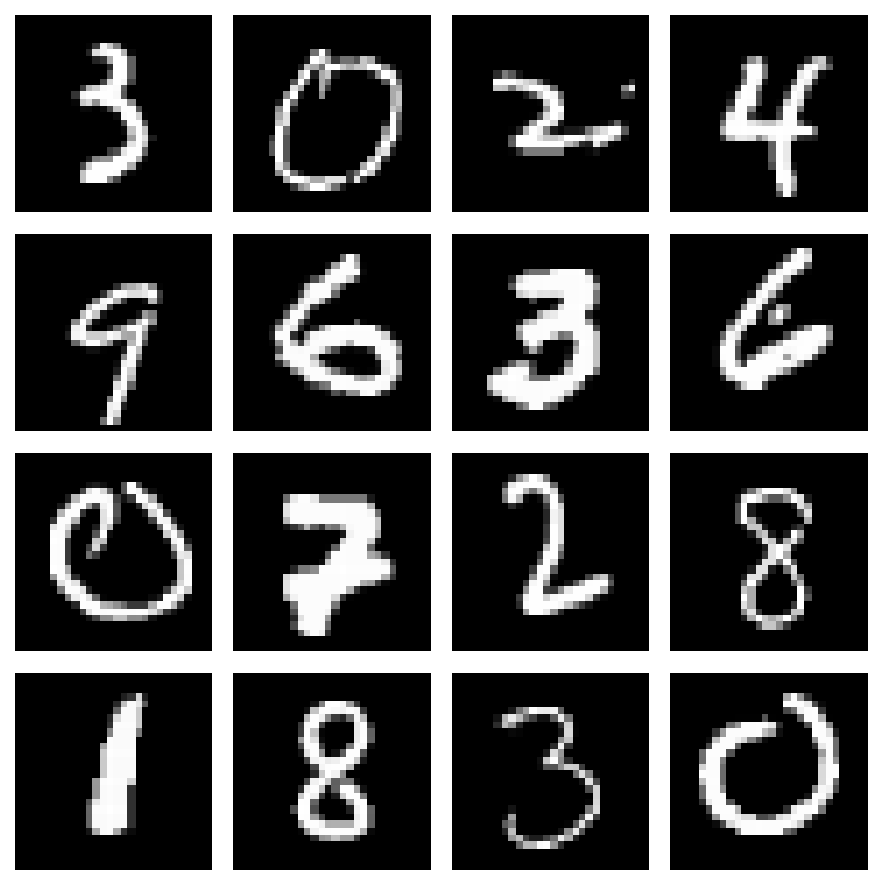
\includegraphics[width=.6\linewidth]{images/mnist.pdf}
      \caption{Random selection of images taken from the MNIST dataset \cite{bib:mnist}. The MNIST dataset consists of 28x28 grayscale images of handwritten digits from 0-9 and has 60000 training examples and 10000 testing examples.}
\label{fig:mnist}
\end{figure}
\FloatBarrier

\begin{figure}[!htb]
    \centering
  \begin{minipage}[b]{.48\linewidth}
      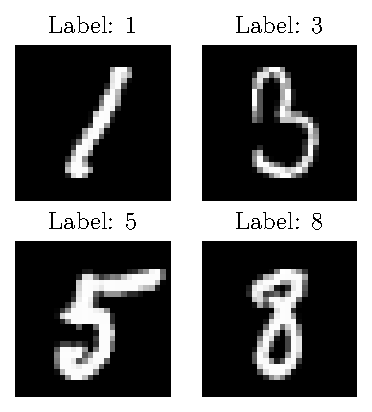
\includegraphics[width=\linewidth]{images/mnist_raw.pdf}
      \subcaption{Original.}
      \label{fig:mnist_dataset_original}
  \end{minipage}
  \begin{minipage}[b]{.48\linewidth}
      
\includegraphics[width=\linewidth]{images/mnist_binarized.pdf}
      \subcaption{Binarized.}
      \label{fig:mnist_dataset_binarized}
  \end{minipage}
  \caption{Part of sample from the original (\subref{fig:mnist_dataset_original}) and binarized (\subref{fig:mnist_dataset_binarized}) MNIST dataset. The original image is the number three and here we show a zoomed-in version(the upper right corner) to make the binarization visible. A LUT network can only do binary classification, so we have to binarize the labels as well. Numbers from 0-4 get the label 0 and numbers from 5-9 get the label 1.}
\label{fig:mnist_dataset}
\end{figure}
\FloatBarrier

\subsection{Experiments from paper}
We construct a LUT network with five hidden layers and 1024 LUTs per hidden layer. Every LUT in the network takes eight bits as input. Construction of the network is performed using the training set with 60000 samples and after training we validate on the test set with 10000 samples. The code is written by ourselves in Python using the package Numpy \cite{bib:harris2020array} for matrix operations. Similar to other machine learning packages, a LUT network object with provided arguments is first created and methods like \hl{\texttt{.train()}} and \hl{\texttt{.predict()}} allows the user to work with the LUT network at a high level. The code is available on GitHub \cite{bib:lut_github}. We obtain a training accuracy of 0.89 and a test accuracy of 0.87 which are the exact results from \cite{bib:chatterjee2018learning}. Note that the results are way above 0.5 meaning some learning had taken place. The way the LUT network is defined, every individual LUT already gives a prediction on the example passed to the network. That means we can compute the accuracy of every LUT in the network. Figure~\ref{fig:ex1_depth_performance} visualizes the training accuracy dependent on the layer. Each point represents the mean training accuracy over the respective layer and the total height of the error bars are two standard deviations. We can see that with increasing layer number, the accuracy goes up and the standard deviation goes down until it reaches zero at layer six because there is only one LUT in the last layer. Increasing performance with increasing depth reminds us of neural networks where adding more layers is a heuristic to increase performance.

\begin{figure}[!htb]
    \centering
    \includestandalone[]{standalone/lut/depth_performance}
    \caption{Training accuracy dependent on the layer for an 8-LUT network with five hidden layers (six is the output layer with just one LUT) and 1024 LUTs per hidden layer, trained on the Binary-MNIST dataset using our own code \cite{bib:lut_github}. The points represent the mean over the respective layer with two standard deviations as total height of the error bars. Similar to neural networks, we can see that performance increases with increasing depth. These results are our own and are almost identical to \cite{bib:chatterjee2018learning}.}
\label{fig:ex1_depth_performance}
\end{figure}
\FloatBarrier

\noindent The bit-size of the LUTs (denoted by $\delta$ in Algorithm~\ref{alg:LUT}) is a crucial hyperparameter. In another experiment, \cite{bib:chatterjee2018learning} varies the bit-size from two to 16 with steps of two and observes the effect on training and testing accuracy. The rest of the LUT network is the same as before. Figure~\ref{fig:ex1_k_acc} visualizes the results.

\begin{figure}[!htb]
    \centering
    \includestandalone[]{standalone/lut/k_acc_real}
    \caption{Training and testing accuracy on Binary-MNIST when the bit-size of a LUT newtwork with five hidden layers and 1024 LUT per hidden layer is varied. Increasing the bit-size sufficiently drives the training accuracy near perfection. As with machine learning models in general, the testing accuracy goes down with too much complexity, meaning we are overfitting. The underlying data to produce this plot is taken from \cite{bib:chatterjee2018learning}.}
\label{fig:ex1_k_acc}
\end{figure}
\FloatBarrier

\subsection{Varying the number of LUTs per hidden layer} \label{sec:num_luts_per_layer}
Throughout this thesis, we will stick with LUT networks with five hidden layers and 1024 LUTs per hidden layer to stay consistent with \cite{bib:chatterjee2018learning}. We will now invesigate what effect changing only the number of LUTs per hidden layer has. We use an 8-LUT network with five hidden layers and evaluate the accuracy at $2^i$ LUTs per layer, where $i = 1, \dots, 12$. The result can be seen in Figure~\ref{fig:num_luts_per_layer}, where Figure~\ref{fig:num_luts_per_layer:num} has an arithmetic scale and Figure~\ref{fig:num_luts_per_layer:num_log} has a logarithmic scale. We can see that going above 512 LUTs per hidden layer does not increase the accuracy anymore. In Section~\ref{sec:lut_network_size} we have seen that the number of LUTs per hidden layer is linearly proportional to the LUT network size on disk. So although not as important as the bit-size, which influences the LUT network size exponentially, reducing the number of LUTs per hidden layer seems like a quick and easy way to reduce LUT network size, especially if the performance does not drop.

\begin{figure}[!htb]
    \centering
  \begin{minipage}[b]{.45\linewidth}
    \resizebox {1\textwidth} {!} {
    \includestandalone[]{standalone/lut/nlpl_num}
    }
    \subcaption{Arithmetic scale.}
    \label{fig:num_luts_per_layer:num}
  \end{minipage}
  \begin{minipage}[b]{.45\linewidth}
    \resizebox {1\textwidth} {!} {
    \includestandalone[]{standalone/lut/nlpl_num_log}
    }
    \subcaption{Logarithmic scale.}
    \label{fig:num_luts_per_layer:num_log}
  \end{minipage}
  \caption{Accuracy of an 8-LUT network with five hidden layers dependent on the number of LUTs per hidden layer, where (\subref{fig:num_luts_per_layer:num}) provides an arithmetic scale and (\ref{fig:num_luts_per_layer:num_log}) provides a logarithmic scale. Increasing the number of LUTs per hidden layer above 512 has no effect on the accuracy.}
\label{fig:num_luts_per_layer}
\end{figure}
\FloatBarrier

\subsection{Summary}
We introduced the concept of LUTs, which are classifiers working entirely in binary, from \cite{bib:chatterjee2018learning} by walking through a small example. A single LUT cannot grasp complex information and is limited in bit-size due to computational constraints, thus we considered LUT networks that are made of many individual LUTs. Using a binarized version of the MNIST dataset, which we call Binary-MNIST, we recreate one experiment from \cite{bib:chatterjee2018learning}, where our results match the ones from the paper. We also made ourselves aware that the bit-size influences the LUT (and thus LUT-network) size exponentially and that the number of LUTs per hidden layer can sometimes be reduced, resulting in a smaller size and almost no performance drop.
